\documentclass[a4paper,12pt]{article}
\usepackage[utf8]{inputenc}
\usepackage{graphicx}
\usepackage{subcaption}
\usepackage{amsmath}
\usepackage{amsfonts}
\usepackage{amssymb}
\usepackage{hyperref}
\usepackage{geometry}
\usepackage{textcomp}
\usepackage{listings}
\usepackage{float}
\usepackage{booktabs}

\geometry{a4paper, margin=1in}

\title{Smart Pacer}
\author{Lorenzo Gandini \\ Internet of Things \\ University La Sapienza \\ A.Y. 2024/2025}
\date{\today}

\begin{document}

% Copertina
\maketitle

\newpage

% Table of Contents
\tableofcontents
\newpage

\section{Abstract}\label{abstract}
Highly motivated runners, from elite to amateurs, soon discover that rigid training plans treat every day as equal—even though sleep, nutrition, hormonal cycles, stress, and travel routinely shift physiological readiness. On a “bad day” an athlete may struggle to complete a prescribed 10 × 1 min Z5 fartlek, while on a “good day” the same session leaves untapped potential.  
\textbf{Smart Pacer} tackles this mismatch by casting second-by-second pacing as a finite-horizon \emph{Markov Decision Process} and solving it with tabular \emph{Q-learning}. 

Each second the agent analyzes a compact environment defined by heart-rate zone, power zone, fatigue, phase of the workout, and slope of the ground, and selects one of three intuitive actions: \emph{accelerate}, \emph{hold}, or \emph{ease}. A multi-term reward function was defined inside the simulation environment to maximize the benefit from each training session.

The model was trained using Q-learning to optimize the reward across different tested parameters, ensuring adaptability to various athlete profiles and workout types. Policies are trained off-line across four canonical workouts (fartlek, progression, endurance, recovery) and three athlete archetypes, then deployed on-line via a 1 Hz MQTT stream that simulates what a smartwatch could prompt in a real-life scenario.

Additionally, a video simulation was developed to visualize athletes' performances on different GPX tracks with the defined training programs, dynamically showing fatigue levels throughout each session.


\section{Formalization of the Markov Decision Process}\label{sec:methodology}
The pacing problem is formalised as a finite Markov Decision Process  
\[
\langle \mathcal{S},\; \mathcal{A},\; \mathcal{P},\; r,\; \gamma \rangle,
\]
where  
\begin{itemize}
  \item \(\mathcal{S}\) is the state space, a tuple of seven components that capture the athlete’s physiological and contextual status.
  \item \(\mathcal{A}\) is the action set, consisting of three discrete commands: \emph{slow down}, \emph{keep going}, and \emph{accelerate}.
  \item \(\mathcal{P}(s'|s,a)\) is the transition dynamics, which describe how the state evolves given an action.
  \item \(r(s,a)\) is the reward function, which quantifies the desirability of each state–action pair.
  \item \(\gamma\) is the discount factor, controlling how future rewards are valued relative to immediate ones.
\end{itemize}

The MDP is implemented in the \texttt{RunnerEnv} class, which simulates the athlete's workout environment and decision-making process. The agent interacts with this environment by observing the current state, selecting an action, and receiving a reward while transitioning to a new state.

\begin{figure}[H]
\centering
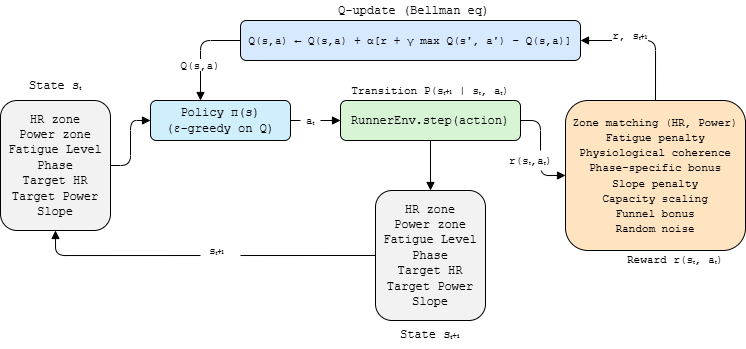
\includegraphics[width=0.99\textwidth]{images/draw_mdp.png}
\caption{Schema of the Markov Decision Process (MDP) for the pacing problem. The agent observes the current state \(s\), selects an action \(a\), and receives a reward \(r\) while transitioning to a new state \(s'\). The process is repeated, allowing the agent to learn an optimal policy over time.}
\label{fig:mdp_diagram}
\end{figure}

\subsection{State space \(\mathcal{S}\)}\label{subsec:state_space}
The states should encapsulate the athlete's physiological state in a specific moment, which is defined by the training program and the context of where the athlete is running. The components of the state space \(\mathcal{S}\) are summarised in Table~\ref{tab:state_space}.
\begin{table}[H]
\centering
\begin{tabular}{@{}lll@{}}
\toprule
\textbf{Component}        & \textbf{Meaning}                                        \\ \midrule
\verb|Heart Rate|         & Instantaneous heart-rate zone (Z1–Z5)                   \\
\verb|Power Zone|         & Instantaneous power zone (Z1–Z5)                        \\
\verb|Fatigue|            & Categorical fatigue (\emph{low/medium/high})            \\
\verb|Phase|              & Workout phase (warm-up, push, recover, cool-down)       \\
\verb|Target HR_zone|     & HR targets of current training segment                           \\ 
\verb|Target Power_zone|  & Power targets of current training segment                        \\
\verb|Slope|              & Terrain label (\emph{uphill/flat/downhill})             \\ \bottomrule
\end{tabular}
\caption{State space \(\mathcal{S}\) components.}
\label{tab:state_space}
\end{table}

\subsection{Action set \(\mathcal{A}\).}
The three admissible actions that an athlete can take during a workout are defined as:
\begin{itemize}
  \item \texttt{slow down} – reduce pace to lower heart rate and power.
  \item \texttt{keep going} – maintain current pace, allowing physiological drift.
  \item \texttt{accelerate} – increase pace to raise heart rate and power.
\end{itemize}

\subsection{Transition dynamics \(\mathcal{P}\)}
The most intricate component of the MDP is the definition of the state–transition kernel, i.e.\ how the athlete's physiological and contextual state evolves once an action is taken. In my simulation, this logic is encapsulated in \verb|RunnerEnv.step()|, which invokes four update routines every second, in the following order:

\begin{itemize}
  \item \verb|_update_power_zone(action)| – the chosen action (\emph{slow down}, \emph{keep going}, or \emph{accelerate}) instantaneously shifts the target wattage, and therefore the power zone. In real life, when you accelerate, your power output increases immediately; when you slow down, it drops right away.
  
  \item \verb|_update_hr_zone(action)| – this function updates the target heart rate zone based on the selected action. Unlike power, heart rate is a lagged variable: it does not change instantaneously, but drifts gradually toward the target zone. This models how the cardiovascular system responds over time.

  \item \verb|_update_fatigue(action)| – a dual-process model accumulates or dissipates fatigue depending on the heart rate, power zone, current workout phase, and the athlete's profile (elite, runner, or amateur).

  \item \verb|_advance_segment()| – the global time index is incremented, the active workout segment is updated accordingly, and the current slope level is recalculated from the GPX elevation trace.
\end{itemize}


Applied sequentially, these rules deterministically map the current pair \((s,a)\) to a unique next state \(s'\) at a granularity of 1 s; stochasticity is confined to the reward function, which injects small uniform noise to break ties.

\subsubsection{Reward function \(r(s,a)\)}
The reward function, together with the \verb|_update_fatigue(action)| routine (see~ \ref{subsubsec:fatigue}), forms the core of the simulator’s logic. These components determine how the agent is incentivised to follow the training plan while accounting for the athlete’s physiological state. The reward function is implemented in the \verb|compute_reward()| method of \verb|runner_env.py|, and outputs a scalar value that quantifies the agent’s performance in the current state and it's given by the sum of eight domain-specific terms:

\begin{itemize}
  
  \item \textbf{Zone–matching accuracy} - the absolute distance between the current and target HR / power zones is mapped to a piece-wise score \(\{+2.0,+0.5,-1.0,-2.5,-4.0\}\); HR and power contributions are then blended as \(0.4\,r_{\text{HR}} + 0.4\,r_{\text{Power}}\).

    \item \textbf{Fatigue management} – We maintain a continuous \verb|fatigue_score| \(f\in[0,10]\) whose dynamics are:
  \[
    \text{if phase}\in\{\text{recover},\text{cooldown}\}:\quad
      f \leftarrow \max\bigl(\mathrm{floor},\,f\,e^{-k}\;-\;d(f)\bigr),
  \]
  where
  \begin{itemize}
    \item \(k = 0.05 \times \text{fitness\_factor}\),
    \item \(d(f) = 0.1 \times \text{fitness\_factor}\times \sigma(f)\),
    \item \(\sigma(f) = 1/\bigl(1 + e^{-10\,(f-5)}\bigr)\),
    \item \(\mathrm{floor} = 0.1 \times \text{fitness\_factor}\).
  \end{itemize}
  In active phases (warm-up, push) \(f\) instead accumulates based on HR-zone gain constants, time in high zones, power coupling, FTP-scaling and session-type modifiers, then is clamped to \([0,10]\).  
  Finally, we classify \(f\) into \emph{low}/\emph{medium}/\emph{high} fatigue by comparing it against the 33rd and 67th percentiles of its own recent history, so that the medium/high labels adapt in real time to the athlete’s current strain.


  \item \textbf{Physiological coherence} – The agent computes \(\Delta_Z=\lvert Z_{\text{HR}}-Z_{\text{Power}}\rvert\). If \(\Delta_Z\) does not exceed the athlete-specific tolerance \(\{0.5,1.0,1.5\}\), a bonus of \(+1.0\) is awarded; otherwise a penalty \(-1.0\times(\Delta_Z-\text{tolerance})\) is applied.  This term encourages consistency between cardiovascular strain (HR zone) and mechanical output (power zone) without overpowering the other rewards.

  \item \textbf{Phase–action consistency} – This function reward the agent for taking actions that are consistent with the current phase of the workout.  For example, in the \emph{warm-up} phase, accelerating while still below the target HR is mildly encouraged \((+0.5)\), while braking is discouraged (-1); in the \emph{recover} phase, slowing down from supra-threshold HR receives +1 while accelerating is harshly penalised (-2).:

  \item \textbf{Terrain-aware pacing} – How the decision taken while the slope is changing can have different impact. Accelerating on an
        \emph{uphill} costs -2.0, braking on a \emph{downhill} -0.5; all other combinations are neutral.

  \item \textbf{Capacity scaling} –  The penalty for exceeding the athlete's \(Z_{\text{HR}}\) is attenuated by the efficiency factor (which is defined as \(\min(1,\text{FTP}/(6\,\text{kg}))\) ), so that lighter or fitter athletes are less penalised for visiting high zones as it should be in real-life.
  
  \item \textbf{Dynamic funnel bonus} – The funnel bonus is a dynamic reward that encourages the agent to maintain a precise pacing as the workout progresses.  It is defined as follows:
        \begin{itemize}
          \item During the first half of the workout, the agent receives +2.0 for entering the target zone and +0.5 for remaining inside.
          \item After halfway, the tolerance shrinks to \(\le 0\), meaning that entering the target zone gives +2.0 only once, while remaining inside yields +0.5.
        \end{itemize}
        This promotes sustained precision pacing.

    \item \textbf{Global fatigue decay \& stochasticity} – After summing all partial rewards, we multiply by 
    \[
      1-\min\!\bigl(\tfrac{f}{200},\,0.4\bigr)\,
    \]
    (capping the fatigue penalty at 40\%), and finally add uniform noise \(\mathcal{U}(-0.1,0.1)\) to break ties and mimic real‐world variability.

\end{itemize}

The final scalar is therefore
\[
r = 0.4\,r_{\text{HR}} + 0.4\,r_{\text{Power}}
     + 0.3\,r_{\mathrm{coh}} + 0.2\,r_{\mathrm{phase}}
     + r_{\mathrm{fatigue}} + r_{\mathrm{cap}}
     + r_{\mathrm{slope}} + r_{\mathrm{fun}},
\]
followed by the multiplicative decay and noise injection, as visible at the end of the \texttt{compute\_reward} method in \texttt{runner\_env.py}.


\subsubsection{Fatigue model}\label{subsubsec:fatigue}
The fatigue model implements a dual-process system: 

\begin{itemize}
    \item \textbf{Recovery/Cooldown Phases:} During these phases, fatigue dissipates through a combination of exponential and sigmoid decay, reflecting the natural recovery process. The decay rate and minimum fatigue floor are modulated by the athlete's fitness factor, ensuring that fitter athletes recover more efficiently. Constants are used to control the rate of decay and to prevent fatigue from dropping below a realistic minimum.
    \item \textbf{Warmup and Push Phases:} In active phases, fatigue accumulates based on the current heart rate (HR) and power zones. The accumulation rate is determined by zone-specific gain constants, which are further adjusted for the type of training session (e.g., interval, fartlek, endurance), the athlete's functional threshold power (FTP), and the time spent in high-intensity zones. Additional scaling is applied if both HR and power are in high zones, and a small random noise is introduced to simulate physiological variability.
    \item The resulting fatigue score is capped to \([0,10]\) and then discretized (low/medium/high) using real‐time percentiles of its history, ensuring the labels always reflect the athlete’s current relative fatigue.
\end{itemize}



\newpage
\section{General settings}\label{sec:settings}
\subsection{Training Programs}
The training programs are defined as follows and they are the typical training sessions that a runner would do during his weekly training plan:
\begin{itemize}
  \item \textbf{Fartlek} – Represent a variable-intensity workout where the athlete alternates between high and low intensity segments, typically in a short time alternation pattern.
  \item \textbf{Progression} – A typical workout where the athlete gradually increases the pace over a set distance or time, starting at a comfortable speed and finishing at a faster pace.
  \item \textbf{Endurance} – A long, steady-state run at a moderate pace, designed to build aerobic capacity and endurance.
  \item \textbf{Recovery} – A low-intensity workout aimed at promoting recovery after a hard training session, typically involving easy running or walking, but with a focus on maintaining the athelte moving with a low heart rate and minimizing fatigue.
\end{itemize}
All these workouts are defined in the \texttt{trainings.json} file.

\subsection{Athlete Archetypes}
The athlete archetypes are defined by their physiological parameters like the heart rate value at rest, the maximal heart rate able to reach and the weight. There are also two \texttt{fitness-related} values: 
\begin{itemize}
\item \textbf{FTP} – Functional Threshold Power (FTP) is a key metric used to define an athlete's performance profile. It represents the highest average power an athlete can sustain for about 60 minutes and is crucial for estimating personalized training zones and overall aerobic capacity. While FTP is most commonly associated with cycling, it is also relevant in running and other endurance sports. Because not every athlete knows their FTP, many fitness apps and smartwatches can estimate this value automatically by analyzing data from multiple workouts, regardless of the activity type. This makes FTP a practical and widely accessible measure for assessing and tracking athletic performance.
\item \textbf{Fitness factor} – A value that represents the athlete's fitness level, which is into the range of 0,7 for an elite athlete, up to 1,3 for an amatour athlete. This value is used to determine the athlete's ability to sustain high-intensity efforts, manage fatigue and how well the athlete it's able to recover.
\end{itemize}

The archetypes, defined in the \texttt{athletes.json} file, are the following:
\begin{itemize}
  \item \textbf{Elite} – Represents a highly trained athlete, like olympic runners with a low resting heart rate, high maximum heart rate, and high FTP. This archetype is characterized by its ability to sustain high-intensity efforts and recover quickly.
  \item \textbf{Runner} – Represents an athlete with average training, having typical resting and maximum heart rates, and a moderate FTP. This archetype can handle standard training sessions and recovers at a normal rate. Could be someone who has been training for a while, like several months, but is not at the elite level yet.
  \item \textbf{Amateur} – Represents an untrained or recreational athlete with a high resting heart rate, low maximum heart rate, and low FTP, typical of someone who begins to train. This archetype is characterized by its limited ability to sustain high-intensity efforts and recover slowly, is the one who suffers more advanced programs.
\end{itemize}

\subsection{GPX Track}\label{sec:gpx-track}
Training was performed on a real GPX track of the \textit{Parco degli Acquedotti} in Rome. To probe generalisation, the learned policies were replayed unchanged on two unseen yet topographically comparable routes: a riverside path in \textit{Parco Belfiore} and the \textit{Lago di Mezzo} waterfront loop, both in Mantova. These additional circuits share similar average slope with the first one but differ in curve geometry and surface, allowing verification that the agent’s behaviour is track-agnostic rather than over-fitted to the training venue. The results of all these simulation can be seen in the video folder.



\newpage
\section{Q-Learning Training Experiments}\label{sec:qlearning}

To train the reinforcement learning policy for the agent, was adopted a tabular Q-learning approach. Multiple hyperparameter combinations were tested evaluating their performance through the cumulative reward across episodes and comparing athlete-specific training results.

\subsection{First Experiment: 500 Episodes}
In the initial experiment, training was limited to 500 episodes per combination (reported in table \ref{tab:hyperparameters-500}). This number was chosen to keep training time feasible while still allowing the Q-values to begin stabilizing and reveal early trends in learning performance.

\begin{table}[h!]
  \centering
  \begin{tabular}{l c c c c c}
    \toprule
    \textbf{Config Label} & $\alpha$ & $\gamma$ & $\epsilon_0$ & $\epsilon_{\min}$ & \textbf{decay} \\
    \midrule
    a10\_g95\_e20  & 0.10 & 0.95 & 0.20 & 0.01 & 0.99  \\
    a5\_g95\_e30   & 0.05 & 0.95 & 0.30 & 0.01 & 0.995 \\
    a10\_g99\_e20  & 0.10 & 0.99 & 0.20 & 0.01 & 0.98  \\
    a1\_g95\_e20   & 0.01 & 0.95 & 0.20 & 0.01 & 0.99  \\
    a10\_g90\_e20  & 0.10 & 0.90 & 0.20 & 0.01 & 0.98  \\
    a10\_g95\_e40  & 0.10 & 0.95 & 0.40 & 0.01 & 0.97  \\
    a5\_g99\_e30   & 0.05 & 0.99 & 0.30 & 0.01 & 0.995 \\
    a5\_g90\_e10   & 0.05 & 0.90 & 0.10 & 0.01 & 0.98  \\
    \bottomrule
  \end{tabular}
  \caption{Hyperparameter sets for 500-episode experiments}
  \label{tab:hp-500}
\end{table}


Each configuration was evaluated across the four predefined workouts and the three athlete profiles explained in section \ref{sec:settings}. For each of them was obtained a heatmap of the total rewards (fig. \ref{fig:amateur-500}, \ref{fig:runner-500}, \ref{fig:elite-500} ), representing the agent's performance across the different hyperparameter settings. 
In order to choose the best option, also the convergence of the Q-values was analyzed, which is shown in figures \ref{fig:convergence-500}. The convergence plots show how the Q-values stabilize over time, indicating that the agent is learning effectively.
\begin{figure}[!htbp]
    \centering
    \begin{subfigure}[t]{0.90\textwidth}
        \centering
        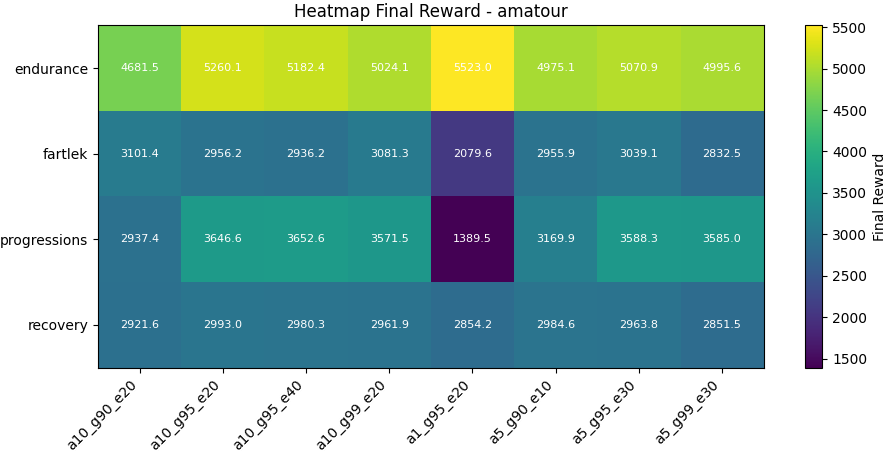
\includegraphics[width=\textwidth]{images/heatmap_final_amatour_500.png}
      \caption{Heatmap for the \textit{amateur} profile after 500 episodes}
    \label{fig:amateur-500}
    \end{subfigure}
    \begin{subfigure}[t]{0.90\textwidth}
        \centering
        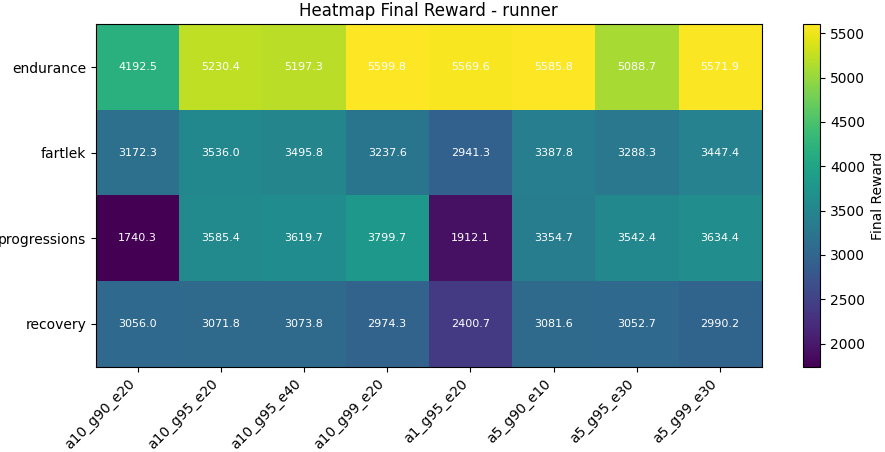
\includegraphics[width=\textwidth]{images/heatmap_final_runner_500.png}
        \caption{Heatmap for the \textit{runner} profile after 500 episodes}
    \label{fig:runner-500}
    \end{subfigure}
    \begin{subfigure}[t]{0.90\textwidth}
        \centering
        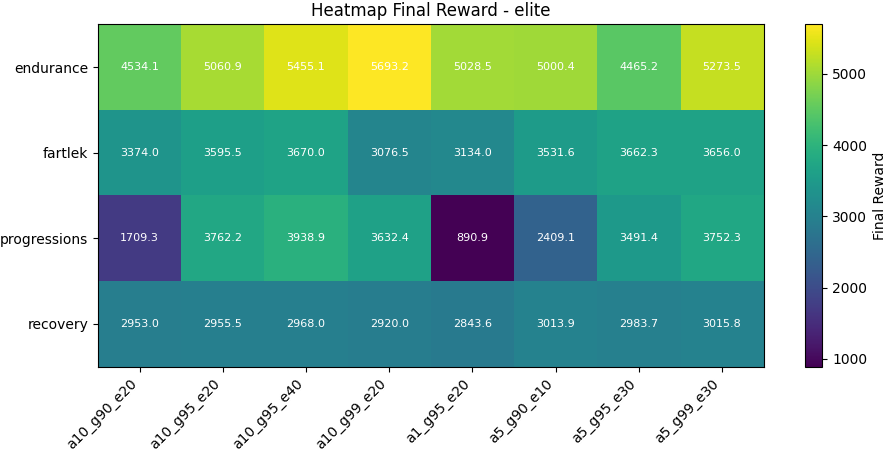
\includegraphics[width=\textwidth]{images/heatmap_final_elite_500.png}
        \caption{Heatmap for the \textit{elite} profile after 500 episodes}
    \label{fig:elite-500}
    \end{subfigure}
    \caption{Heatmaps of total rewards for different athlete profiles after 500 episodes}
\end{figure}

\begin{figure}[!htbp]
    \centering
    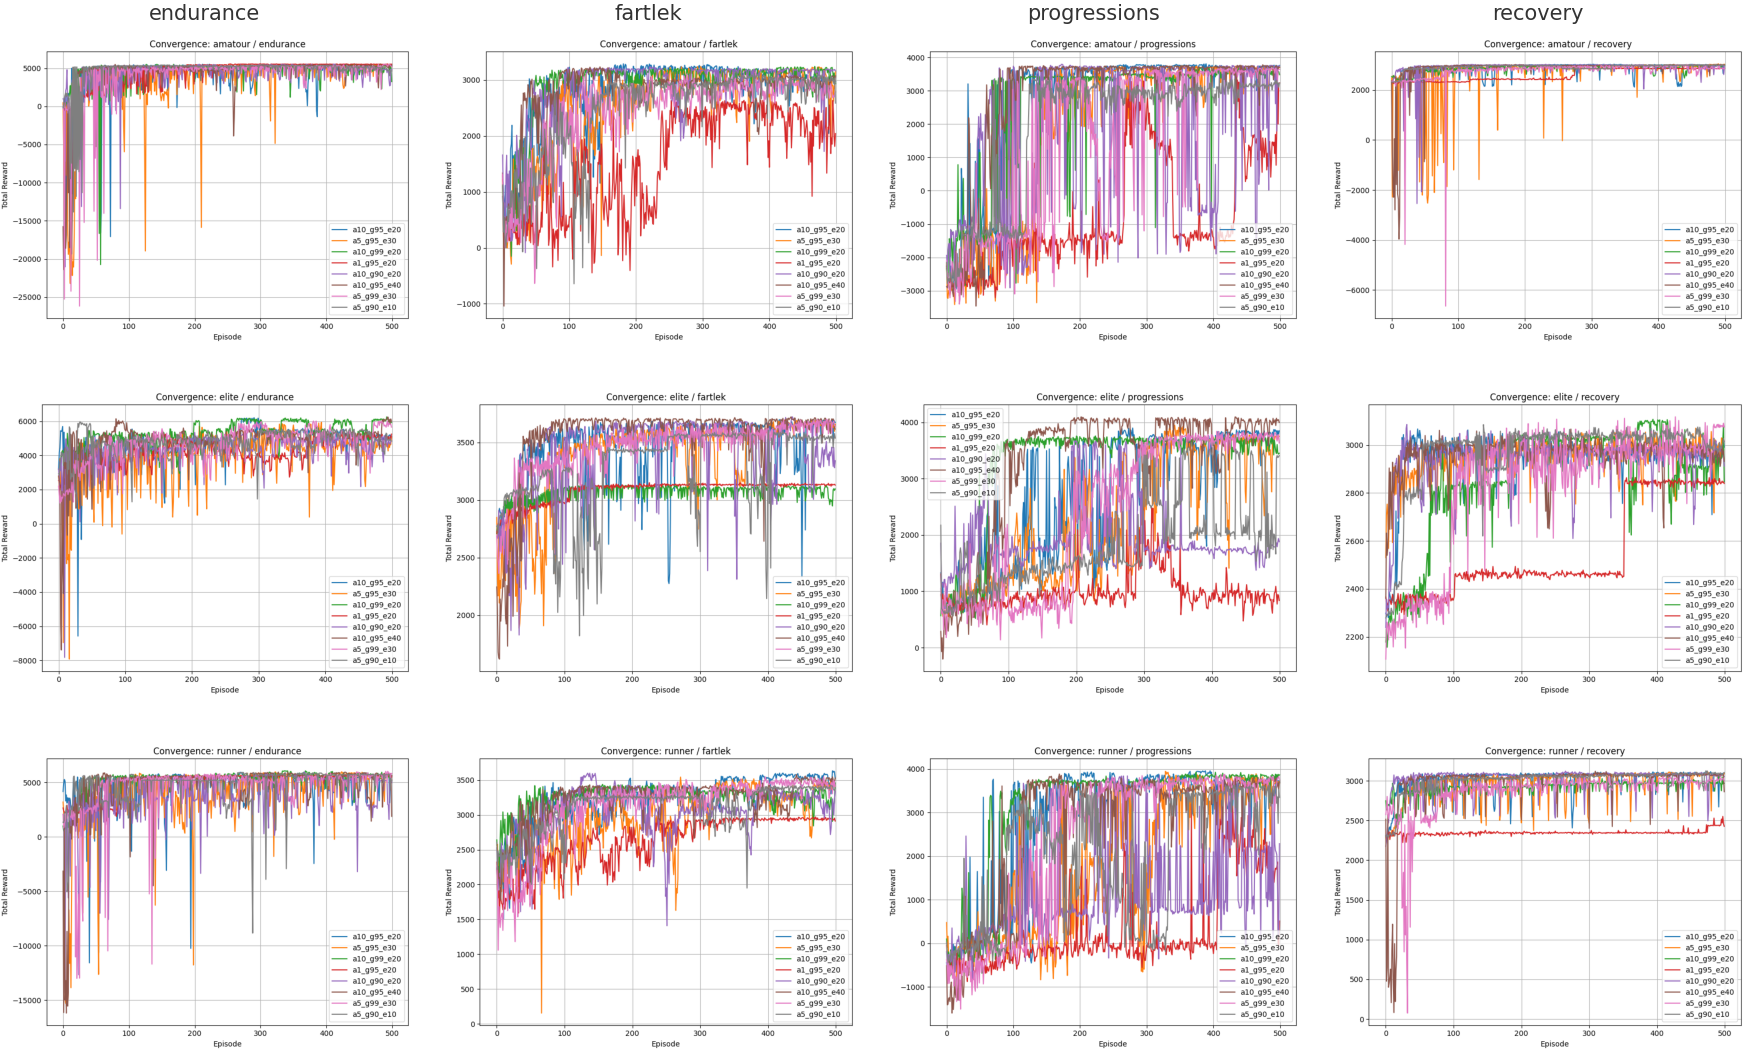
\includegraphics[width=1\textwidth]{images/convergence_grid_500_custom.png}
    \caption{Convergence of Q-values for tested hyperparameter configurations after 500 episodes.}
    \label{fig:convergence-500}
\end{figure}


Table~\ref{tab:hp-500} shows that most settings achieve a stable plateau well before the 500-episode mark; however, overly aggressive ``future-looking'' combinations (e.g., $\gamma = 0.99$) or highly exploratory starts (e.g., $\epsilon = 0.40$) sometimes dip late in noisy workouts like Fartlek and Progressions. The heatmaps in Figures~\ref{fig:amateur-500}--\ref{fig:elite-500} make it clear that \texttt{a10\_g95\_e20} consistently delivers the highest final rewards across all athlete types. For an \textit{elite} runner, who physiologically can sustain high intensity with minimal fatigue, that configuration tops the Endurance cell at about 5500 total reward, while still keeping fatigue low in recovery phases.

In contrast, an \textit{amateur} is expected to accumulate fatigue almost everywhere; indeed, only \texttt{a10\_g95\_e20} pushes them into medium fatigue zones without driving them into unsustainable high-fatigue levels. Less balanced choices either converge more slowly or produce erratic fatigue spikes, making them less reliable for a real-time pacing assistant.

\subsection{Second Experiment: 1000 Episodes}

To validate the consistency of the best configurations, or confirm that \texttt{a10\_g95\_e20} is the best combination, a reduced subset of hyperparameter combinations (based on the first test results) was run with 1000 episodes. 
This longer training period allowed more stable policy convergence and finer reward differentiation. 
Even if most of the convergence of the Q-values was already nearly reached, with 1000 episodes the agent was able to explore the state-action space further and refine its policy. 
The values of the hyperparameters used in this second experiment are shown in Table~\ref{tab:hp-1000}.

\begin{table}[h!]
  \centering
  \begin{tabular}{l c c c c c}
    \toprule
    \textbf{Config Label} & $\alpha$ & $\gamma$ & $\epsilon_0$ & $\epsilon_{\min}$ & \textbf{decay} \\
    \midrule
    a5\_g90\_e10   & 0.05 & 0.90 & 0.10 & 0.01 & 0.98  \\
    a10\_g95\_e20  & 0.10 & 0.95 & 0.20 & 0.01 & 0.99  \\
    a10\_g99\_e20  & 0.10 & 0.99 & 0.20 & 0.01 & 0.98  \\
    a5\_g95\_e30   & 0.05 & 0.95 & 0.30 & 0.01 & 0.995 \\
    \bottomrule
  \end{tabular}
  \caption{Hyperparameter sets for 1000-episode experiments}
  \label{tab:hp-1000}
\end{table}

\begin{figure}
    \centering
    \begin{subfigure}[t]{0.32\textwidth}
        \centering
        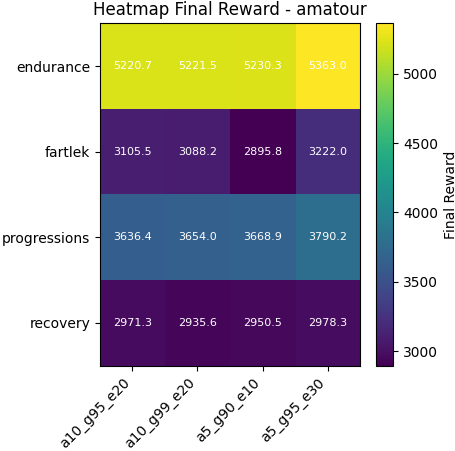
\includegraphics[width=\textwidth]{images/heatmap_final_amatour_1000.png}
      \caption{\textit{amateur} profile }
    \label{fig:amateur-1000}
    \end{subfigure}
    \begin{subfigure}[t]{0.32\textwidth}
        \centering
        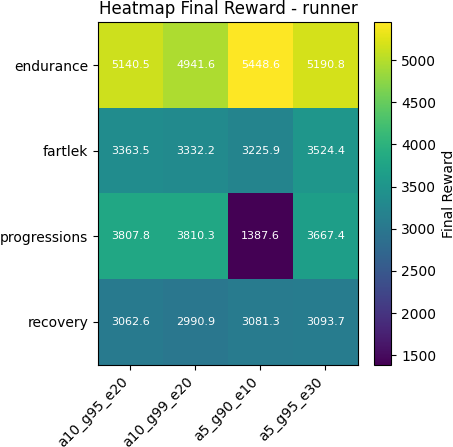
\includegraphics[width=\textwidth]{images/heatmap_final_runner_1000.png}
        \caption{\textit{runner} profile }
    \label{fig:runner-1000}
    \end{subfigure}
    \begin{subfigure}[t]{0.32\textwidth}
        \centering
        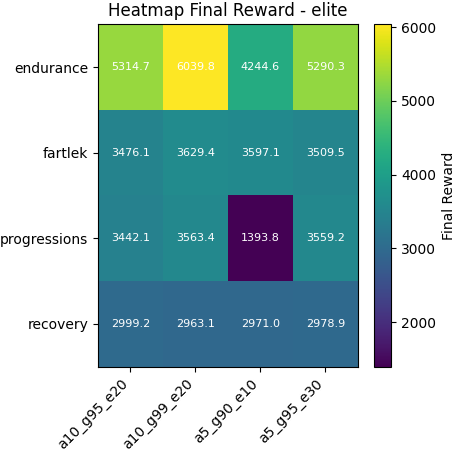
\includegraphics[width=\textwidth]{images/heatmap_final_elite_1000.png}
        \caption{\textit{elite} profile }
    \label{fig:elite-1000}
    \end{subfigure}
    \caption{Heatmaps of total rewards for different athlete profiles after 1000 episodes}
\end{figure}

\begin{figure}[t]
    \centering
    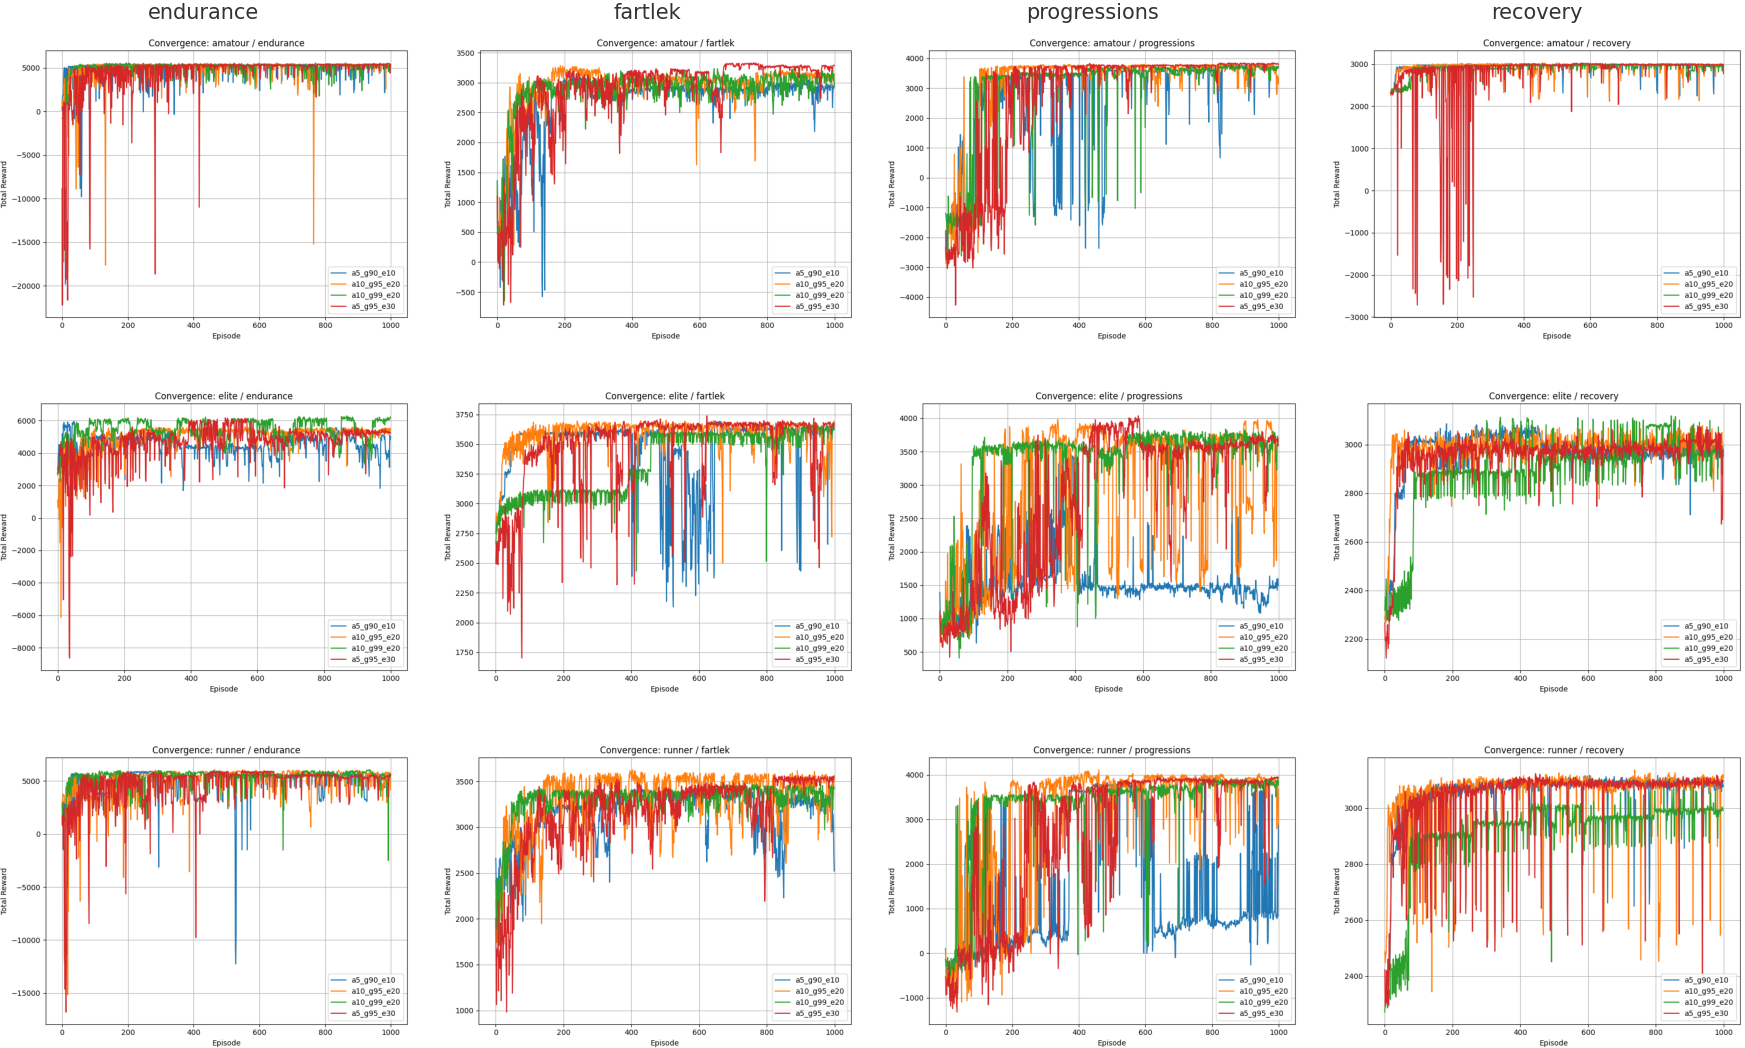
\includegraphics[width=0.99\textwidth]{images/convergence_grid_1000_custom.png}
    \caption{Convergence of Q-values for tested hyperparameter configurations after 1000 episodes.}
    \label{fig:convergence-1000}
\end{figure}

As shown in Figure~\ref{fig:convergence-1000}, all configurations now achieve very smooth, late-episode plateaus, with only minor oscillations remaining in the more complex workouts (\textit{fartlek}, \textit{progressions}). The heatmaps in Figures~\ref{fig:amateur-1000}~to~\ref{fig:elite-1000} reveal that \texttt{a10\_g95\_e20} not only retains its lead but widens the gap: it delivers the highest total reward for every athlete profile. From a physiological standpoint, our \textit{elite} runners benefit most from the balanced focus on immediate and future rewards, achieving peak performance in \textit{endurance} without unnecessary fatigue spikes in recovery. Conversely, \textit{amateurs}, who naturally accumulate fatigue more quickly, see a gentler fatigue profile under this configuration, avoiding severe high-fatigue states even in the toughest segments. The extended training thus confirms \texttt{a10\_g95\_e20} as the most robust and physiologically coherent choice across all scenarios.

\section{Final Q-tables and Policies}
After choosing the best hyperparameters (\texttt{alpha=0.1, gamma=0.95, epsilon=0.2}), a final run with 2000 episodes was performed to ensure the Q-values were fully converged and stable. This final run allowed the agent to refine its policy further, ensuring that it could make optimal decisions during each training session.
Different athletes, in the end, respond to the same training program in different ways, adapting their pace and heart rate according to their physiological parameters. The agent is able to adapt its behaviour to the athlete's profile, ensuring that the training is tailored to the athlete's needs.
A demonstration of the agent's performance can be seen in the video folder (and also in the figures below \ref{fig:video-amator}, \ref{fig:video-runner}, \ref{fig:video-elite}  ), where the agent is shown running in all possible combinations of \texttt{athlete}, \texttt{training program}, and also \texttt{different track} and below there 

\begin{figure}[h!]
    \centering
    \begin{subfigure}[t]{0.31\textwidth}
        \centering
        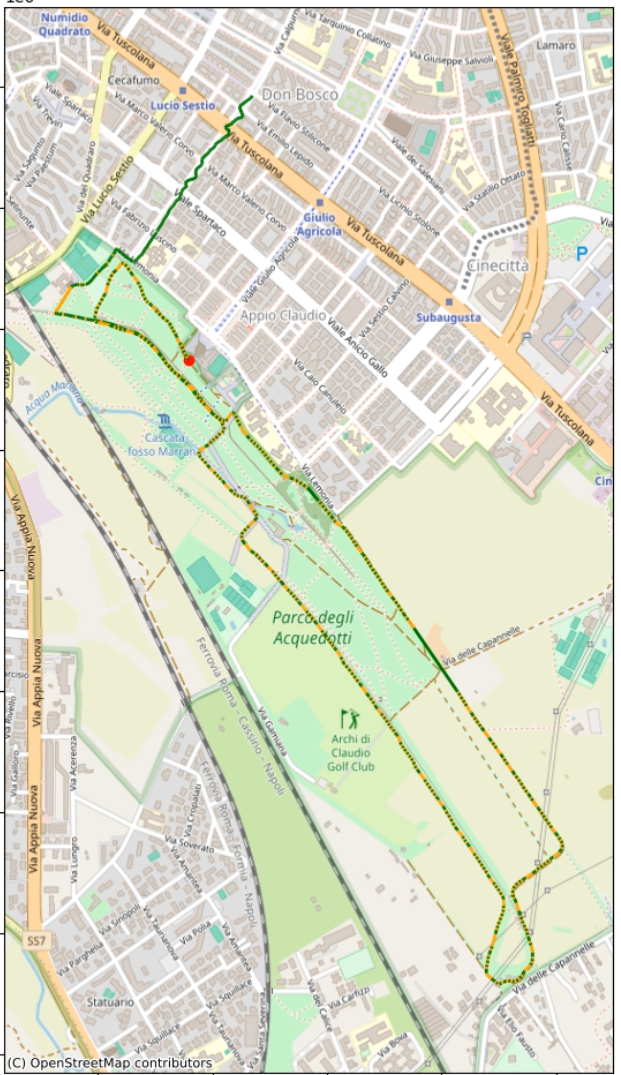
\includegraphics[width=\textwidth]{images/amatour-roma.png}
      \caption{\textit{amateur} simulation at Parco degli Acquedotti, Rome}
    \label{fig:video-amator}
    \end{subfigure}
    \begin{subfigure}[t]{0.305\textwidth}
        \centering
        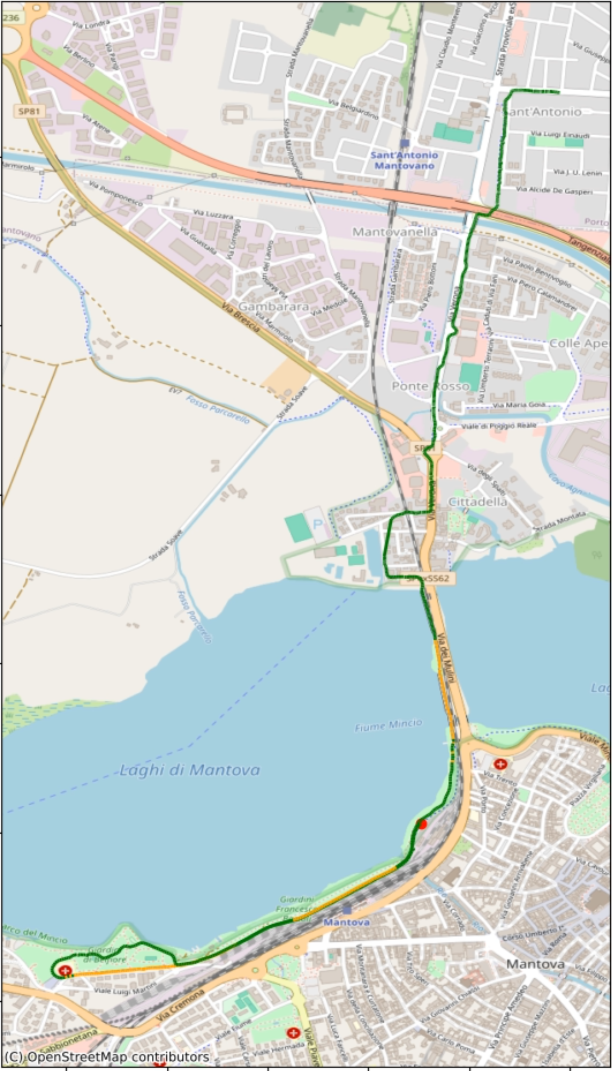
\includegraphics[width=\textwidth]{images/runner-belfiore.png}
        \caption{\textit{runner} simulation at Parco Belfiore, Mantova of a progression training program}
    \label{fig:video-runner}
    \end{subfigure}
    \begin{subfigure}[t]{0.31\textwidth}
        \centering
        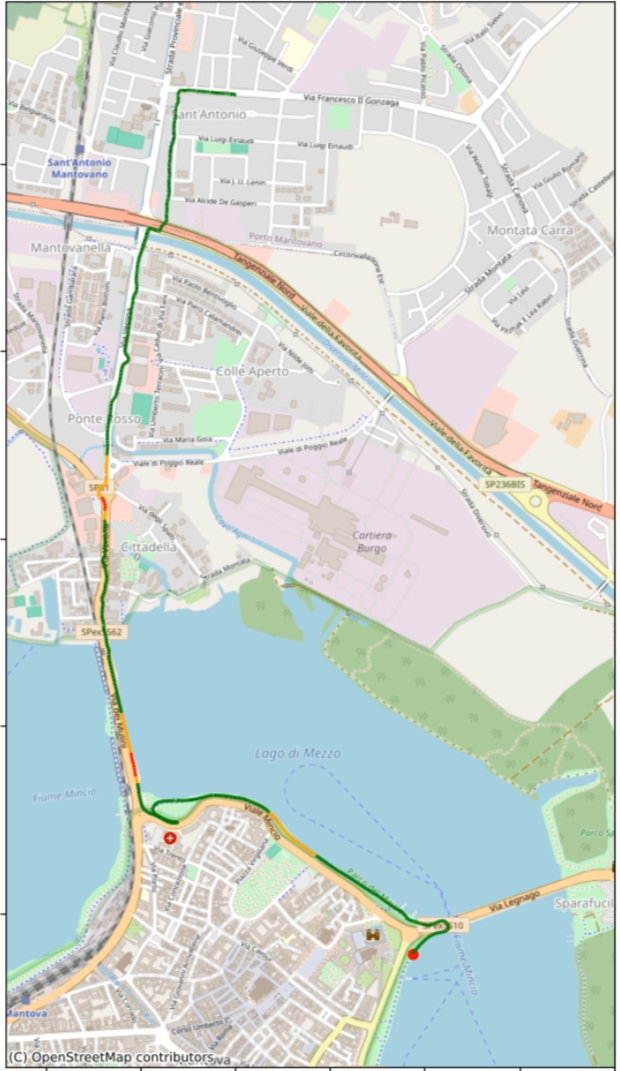
\includegraphics[width=\textwidth]{images/elite-fartlek.png}
        \caption{\textit{elite} simulation of the fartlek training program at Mantova, between the three lakes}
    \label{fig:video-elite}
    \end{subfigure}
    \caption{Screenshots from video simulations of the agent's performance across different athlete profiles and training programs. Red lines means high fatigue, yellow means medium fatigue, and green means low fatigue}
\end{figure}



\newpage
\section{MQTT Communication}\label{sec:mqtt-communication}
To simulate communication between the smartwatch application (acting as the smart pacer) and the user, an MQTT session was established. This setup allows the user to send data to the smartwatch app, which processes the information (by running the RunnerEnv) and provides feedback, including suggested actions.

\subsection{MQTT Messages}
The communication occurs over the topic \texttt{smartpacer/action} using the public broker \texttt{broker.emqx.io}.

The payload of each MQTT message is a JSON object containing the following fields:
\begin{itemize}
  \item \texttt{second}: the current second of the workout;
  \item \texttt{phase}: the current phase of the workout;
  \item \texttt{fatigue}: the athlete's current fatigue level;
  \item \texttt{action}: the action suggested by the smart pacer, which can be one of \emph{accelerate}, \emph{hold}, or \emph{ease}.
\end{itemize}

Each field is represented as a string, accompanied by a relevant emoji to enhance the user experience.

An example of the messages are shown in figures .

% \ref{fig:mqtt_message_example}.



% \begin{figure}[H]
%   \centering
  
%   \begin{subfigure}[position][height][inner pos]{width=0.2\textwidth}
%     \centering
%     \includegraphics[width=\textwidth]{images/mqtt_message_example_emoji.png}
%     \caption{Example of an MQTT message with emojis.}
%     \label{fig:mqtt_message_example_emoji}
%   \end{subfigure}

%   \begin{subfigure}[position][height][inner pos]{width=0.2\textwidth}
%     \centering
%     \includegraphics[width=\textwidth]{images/mqtt_message_example_emoji.png}
%     \caption{Example of an MQTT message with emojis.}
%     \label{fig:mqtt_message_example_emoji}
%   \end{subfigure}

%   \caption{Example of an MQTT message sent by the smart pacer.}
%   \label{fig:mqtt_message_example}
% \end{figure}

  

\newpage
\newpage\section{Challenges and Future Improvements}\label{sec:limitations}
\section{Limitations and Future Improvements}\label{sec:limitations}

\subsection{State-space explosion}
The current Markov model already spans seven discrete variables, yielding several thousand reachable combinations.  Extending realism would require additional factors — e.g.\ \emph{weather} (temperature, humidity, wind) and \emph{surface type} (asphalt, track, trail, grass). Although essential for real-world fidelity, every new dimension inflates the state complexity.

\subsection{Richer athlete profiles}
Present profiles depend on basic informations and a FTP valu. A more faithful description would incorporate sex, age, injury history, recent training load, previous-night sleep quality, HRV-derived recovery indices and update them with the evolution of the training process. 
Such metadata would enable session prescriptions that respect female hormonal cycles, age-related recovery kinetics, and cumulative muscle stress.

\subsection{Fatigue and reward refinement}
Fatigue and reward terms were the hardest features to properly develop. In order to be even more realistic and coherent with real life behaviours could be implemented also a \textbf{Injury-risk term}, which will introduce a weekly load delta component that penalises abrupt increases in training load, reducing overuse-injury likelihood.
Another possibl improvement could be the introduction of \textbf{sleep quality} and \textbf{recovery indices} as additional reward terms, which would allow the agent to adapt its pacing strategy based on the athlete's recovery status. This could be particularly useful for athletes with varying sleep patterns or those recovering from intense training sessions.

\subsection{Temporal resolution}
All decisions are issued at 1 Hz. Increasing the control loop to 5–10 Hz — or adopting event-driven updates triggered by rapid HR changes would shorten feedback latency and smooth the athlete's perceived guidance.

\subsection{Personalised on-line learning}
After the first ten sessions, enough data exist to characterise an individual pacing style.  Fine-tuning the policy with a small neural network head (e.g.\ policy-gradient or Soft Actor Critic) on top of the pre-trained Q-table would capture personal patterns without restarting from scratch.  
Meta-learning techniques could further shrink the cold-start phase for new athletes.


\bigskip
Addressing the above points will increase both realism, athlete safety but most importantly will move \emph{Smart Pacer} closer to a deployable digital coach that can adapt to individual needs and conditions, providing a more effective and personalized training experience.

\end{document}
